%%%%%% @TODO PONER TABLA CON TWEETS DE EJEMPLOS



\section{Case Studies}
\label{sec:experimental}

We describe the case studies, the data, and the experiment we performed to
validate our representation.

\subsection{Datasets}

%We follow a similar approach to Kalyanam et al.~\cite{kalyanam2016prediction}.
%
We collected tweets using the Twitter Search API using selected news accounts as
seeds for extracting newsworthy search terms.
%
In particular, given a set of verified news accounts in Twitter (such as
BBCNews, CNN, Al Jazeera, etc.), we identify the most common keywords across
their tweets published every hour, and then we use those keywords as search
terms in the Twitter API.
%\footnote{The full list of news accounts is listed in
%\url{https://github.com/mquezada/twitter-event-detection/blob/master/settings.py}}

% The data collection methodology is as follows. 
% %
% Every hour we fetch the latest tweets for each one of the seed accounts. 
% %
% Our assumption is that if an important event is happening in a certain moment
% in time, then several news accounts will be reporting on that event shortly
% after.
% %
% After the removal of stopwords, punctuation, URLs, hashtags, mentions, and
% converting words to lowercase, we tokenize each headline and find named
% entities, such as person names, locations, product names, organizations, etc.
% %
% This is possible due that the selected accounts generally employ formal
% language in their tweets. 
% %
% Then we find common subsets of tokens across the tokenized headlines, using an
% ad-hoc method resembling frequent itemset mining. 
% %
% Finally, from each common subset, we search for more related tweets in the
% Twitter Search API using the top 3 ranked terms for the next hour until the
% next batch of keywords is extracted. 

% The source code of the data collection methodology is
% available\footnote{\url{https://github.com/mquezada/twitter-event-
% detection/}}.
%
For the case studies, we selected three events of different nature, namely a
terrorist attack (2015 Libya Hotel Attack), a long-lasting event (2014 Oscar
Pistorius Trial), and a natural disaster (2015 Nepal Earthquake).
%
Each event has different scales and levels of redundancy. 
%
We report duration in days (corresponding to the amount of days encompassing at
least 95\% of the tweets), total tweets, retweets (with percentage of total
tweets), and unique resolved URLs (Table~\ref{tab:datasets}).
%
We also report some tweets for each event (Table~\ref{tab:sample}).


\begin{table}[ht!]
  \centering
  \caption{Datasets for case studies.}
  \label{tab:datasets}
  \begin{tabular}{@{}lllll@{}}
  \toprule
  Name                  & Duration & Tweets & Retweets & URLs  \\ \midrule Libya
  Hotel Attack    & 8 days   & $28\,616$ & $12\,280$ (43\%)  & $3\,385$
  \\
  Nepal Earthquake      & 1 day   & $522\,434$ & $363\,102$ (70\%) & $22\,661$
  \\ 
  Oscar Pistorius Trial & 70 days  & $113\,189$ & $26\,307$ (23\%)  & $9\,335$
  \\ \bottomrule
  \end{tabular}
\end{table}


% {\bf 2015 Libya Hotel Attack.} 
% %
% In January 27, 2015, a luxury hotel in Tripoli was attacked by men affiliated
% with
% ISIL.\footnote{\url{https://en.wikipedia.org/wiki/2015_Corinthia_Hotel_attack}
% (Accessed: 2019-01-30)}. % Attackers detonated a car bomb outside the hotel, %
% killed security personel and guests, and took hostages afterwards. We filtered
% % our data using keywords such as {\tt libya}, {\tt luxury}, {\tt hotel}, or
% {\tt % attack}. % The tweets ranged from July 2012 to January 27, 2015. The
% existence of % older tweets is explained by the retrieval of retweets and
% older tweets % mentioning the extracted keywords, although more than 95\% of
% the tweets fall % within one week before or at the day of the attack. The
% dataset consists of $28\,604$ tweets (with $12\,280$ or 43\% of them being
% retweets), 25\,683 different short and $3\,385$ unique URLs after expanding
% the short URLs. 
% %
% We found that 5\,759 short URLs were unable to be resolved (due to be
% inaccessible at the time of the resolution).

% % On the other hand, due to the occurrence of keywords such as {\tt luxury}, %
% several unrelated tweets appeared in the dataset, such as the following:

% % \begin{itemize} % \item Cheers {\tt <mention>}, named Best Luxury Hotel in
% The Netherlands by {\tt <mention>}! % \item New York's dazzling Baccarat Hotel
% opens this March, and it looks set to be a corker % \item What are your
% thoughts on this distinctive new hotel planned for development in China? %
% \end{itemize}

% %%

% {\bf 2015 Nepal Earthquake.} 
% %
% In April 25, 2015, Nepal was struck by a 7.8 $\text{M}_\text{W}$ earthquake,
% killing nearly $9\,000$
% people\footnote{\url{https://en.wikipedia.org/wiki/April_2015_Nepal_earthquake}
% (Accessed: 2019-01-30)}. 
% %
% The dataset consists of $522\,434$ tweets, with the 70\% of them being
% retweets.
% %
% Also, $60\,632$ of the short URLs were unable to be resolved.

% %%

% {\bf 2014 Trial of Oscar Pistorius.} 
% %
% The trial of Oscar Pistorius started on March 3, 2014, and in October, 2014 a
% judge sentenced him for a maximum of 5 years for homicide; in 2015 and 2016 he
% received more
% sentences\footnote{\url{https://en.wikipedia.org/wiki/Trial_of_Oscar_Pistorius}
% (Accessed: 2019-01-30)}.
% % 
% The dataset consists of $113\,189$ tweets, with 23\% of them being retweets.
% %
% Also, $21\,807$ short URLs were unable to be resolved.





\subsection{Experimental setting}

To generate the representation for each event, we discarded all tweets that have
more than two URLs or more than three hashtags, as we consider them as
potentially spam tweets. 
%
Note that some spam tweets may not fall into this filter.
%
We resolved every URL mentioned in the resulting tweets by following redirects. 
%
Even though the tweet meta-data may include the URLs as before they were
shortened by the Twitter platform, they are often shortened by additional
external services (e.g., {\tt bit.ly}) even more than once.
%
Also, we removed all query strings from the URLs, with some exceptions, which
for some sites they are relevant to identify the resource (e.g., {\tt ?id=},
{\tt ?fbid=}, {\tt ?v=}, etc.).

%%

The URLs which co-occurred with two or less other URLs in the same tweets were
considered as topic-specific.
%
Then, we computed the representation for each event by identifying connected
components in the graph of tweets and URLs. We discarded tweets without URL.
%
This resulted in $2\,957$ documents for the Libya event, $20\,984$ for the Nepal
event, and $9\,092$ for the Pistorius event.

%%

We used fastText~\cite{bojanowski2016enriching} to produce dense vectors from
the documents.
%
We choose fastText due to its capability to encode sub-word information into the
embeddings and to encode some out-of-vocabulary words, resulting in better
quality embeddings for rare or uncommon words. 
%
This is useful in the context of social media, as there are many words with
misspellings. 
%
For the generation of document vectors, we took all the tweets in a document,
and obtained the vector of each word in each tweet.
%
Then, we took the sum of the vectors of the words in the document.
%
We trained 300-dimension word embeddings using a dataset of 193 million
event-related tweets (3 billion words) using the aforementioned data collection
methodology.
%
Note that the training phase can be done off-line and is done only once.


\subsection{Validation of sub-topic detection task}

To validate our representation in the case studies, we identified topics in our
events using our representation and using raw tweets.
%%

We produced a set of labels from the tweets in order to have a ground truth for
our experiments. 
%
For this, sixteen people (mainly Computer Science undergrad and grad students)
labeled tweets independently using a custom Web interface. 
%
The interface displayed a tweet and a list of labels, and each user could assign
one or more labels to a tweet, mark the tweet as non relevant, or skip it.
%
Some tweets may refer to more than one sub-topic, and we preferred that users
felt free to assign as many labels as they prefer.
%
We imposed a limit of three evaluations per tweet.
%
We manually generated the list of labels using information from news reports in
the Web.
%
The tweets displayed in the interface were chosen in such a way there were
roughly no underrepresented sub-topics.
%
For this, we manually produced a list of keywords for each label, and for each
label ranked the tweets using Okapi BM25 and shuffled the ranked tweets to be
shown in the interface.
%
Finally, to assign the actual label to a tweet, we selected the most voted
label.
%
This resulted in 401 labeled tweets for the Libya event, 368 for Nepal, and 85
for Pistorius.

%%

To find sub-topics, we ran k-means with different number of clusters, using our
representation and raw tweets.
%
For the baseline, we considered each tweet as a document, that is, we computed
the sum of word vectors for each tweet individually.
%
We report normalized mutual information, purity, and entropy for each event,
using the available labels in both settings (Figure~\ref{fig:results}).
%
Note that the measures were done only on the labeled tweets, that is, as if the
unlabeled tweets did not exist in the clustering solution.


%%

We observe that with under our representation, the clustering outperforms the
baseline in some cases. 
%
In the case of the Nepal event, our representation had better purity, NMI and
entropy. 
%
In the case of Pistorius, the measures are very similar. 
%
However, in the case of Libya, our representation matches the baseline after a
certain number of clusters, except in the entropy measure.
%
And in terms of running time, we observed that k-means under the representation
runs one order of magnitude faster than the baseline (Figure~\ref{fig:times}). 
%
These results suggest that our representation is capable of preserving topical
information about the target event, with reduced time required to identify this
kind of information.
 

\begin{figure}
  \centering
  \begin{subfigure}[b]{0.478\textwidth}
      \centering
      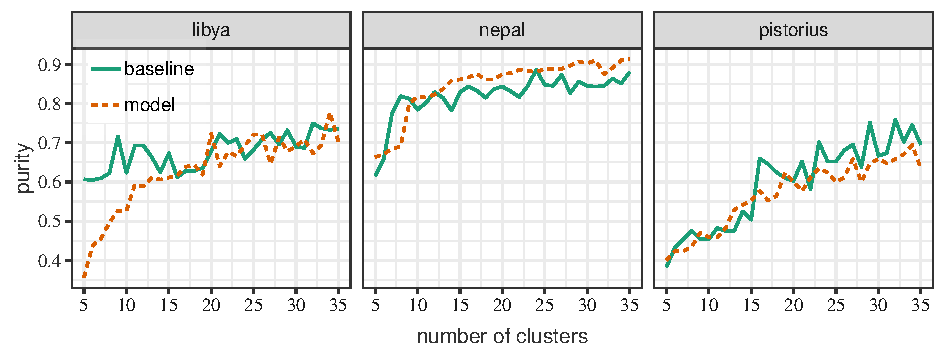
\includegraphics[width=\textwidth]{figures/url-model/purity}
      \caption{Purity.}
  \end{subfigure}%

  \begin{subfigure}[b]{0.478\textwidth}
      \centering
      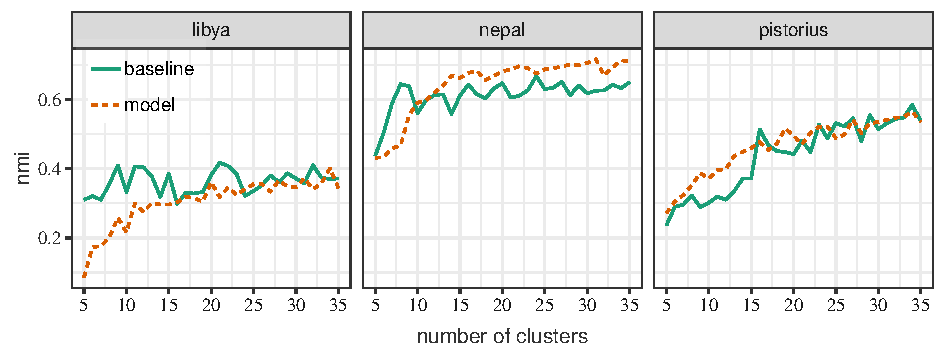
\includegraphics[width=\textwidth]{figures/url-model/nmi} 
      \caption{Normalized Mutual Information.}
  \end{subfigure}

  \begin{subfigure}[b]{0.478\textwidth}
    \centering
    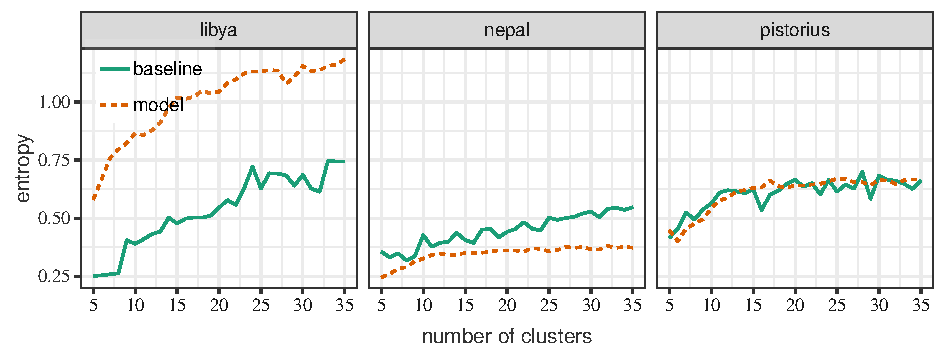
\includegraphics[width=\textwidth]{figures/url-model/entropy} 
    \caption{Entropy.}
  \end{subfigure}

\caption{External clustering measures for target events.}
\label{fig:results}
\end{figure}

\begin{figure}
  \centering
  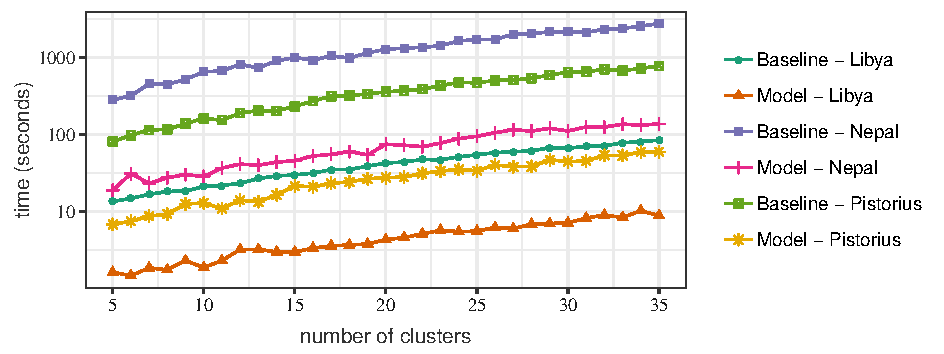
\includegraphics[width=.478\textwidth]{figures/url-model/times}
  \caption{Running times for clustering.}\label{fig:times}
\end{figure}%